% ==============================================================================
% TCC - César Henrique Bernabé
% Capítulo 3 - Zanshin
% ==============================================================================

\chapter{Análise do Metamodelo do \zanshin}
\label{sec-zanshin}

Esta seção trata do processo de reavaliação do metamodelo operacional do sistema \zanshin, anteriormente já apresentado na Figura~\ref{figura-metamodelo-antigo}.

%\vitor{Acho que o título deveria ser modificado para algo que represente mais fielmente o conteúdo da seção.}

% ======================================================================================================
% SUBSEÇÃO Motivação
% ======================================================================================================
%\section{Motivação}
%\label{sec-zanshin-motivacao}
Durante estudos realizados sobre a implementação do \framework \zanshin, foram detectadas algumas oportunidades de melhoria relacionadas principalmente ao metamodelo de objetivos utilizado pelo sistema. A maioria das adequações identificadas referem-se a dois motivos: ou o metamodelo não era restrito o suficiente, deixando que algumas situações indesejadas pudessem ser modeladas; ou o metamodelo não refletia fielmente alguns conceitos de \gore que foram mais bem elaborados em discussões sobre o tema. Então, o metamodelo original foi retrabalhado levando também em consideração as definições propostas pela ontologia \goro, que permitiu definir elementos com mais presição e adicionar restrições que antes não existiam. A Subseção~\ref{sec-zanshin-revisao} trabalha oportunidades de melhoria do metamodelo original, enquanto a Subseção~\ref{sec-zanshin-proposta} demonstra como soluções para essas propostas de melhoria foram elaboradas.

O código fonte da versão original do \zanshin pode ser encontrado em \codigoZanshin, assim como a versão modificada para adequação a nova proposta de metamodelo pode ser encontrada em \codigoZanshin2.

%\vitor{Apresentar as subseções.}

%\vitor{Acho que faltou dizer também que a GORO foi usada como base para a definição do novo metamodelo. Pra isso precisaríamos falar brevemente sobre a GORO no Capítulo~\ref{sec-referencial}...}

% ======================================================================================================
% SUBSEÇÃO Revisão do Metamodelo
% ======================================================================================================
\section{Revisão do Metamodelo}
\label{sec-zanshin-revisao}
A partir da análise de cada elemento do metamodelo antigo, foram encontradas as seguintes oportunidades de melhoria:

\begin{enumerate}
	%1
	\item \textbf{Requirement}: o fato desse elemento estar no topo da hierarquia e todos os outros elementos serem especializações dele faz com que suas características sejam herdadas por todos os outros componentes do modelo. Porém, nota-se que algumas características na verdade são inerentes a apenas alguns elementos. Por exemplo: \textit{Requirement} possui a relação de agregação \textit{Parent} para \textit{Children}, permitindo que cada elemento tenha zero ou um ``Pai'' e um ou vários ``Filhos''. Entretanto, a agregação pai/filho é indesejada nos elementos \awreq, \textit{DomainAssumption} e \textit{QualityConstraint}, visto que esses não são refinados, apenas possuem ``alvos''. \label{p1}
	
	%2
	\item \textbf{DeinableRequirement} e \textbf{Softgoal}: \sofgoal possui o mesmo tipo de comportamento de um \textit{DefinableRequirement} e, portanto, seria esperado que aquele também fosse uma especialização deste. Assim, com essa modificação seria desnecessário a utilização de duas classes (\textit{Requirement} e \textit{DefinableRequirement}) na composição do modelo, que poderiam perfeitamente ser reduzidas a apenas uma. \label{p2}
	
	%3
	\item \textbf{Softgoal} e \textbf{QualityConstraint}: O modelo permite que um \textit{Softgoal} contenha nenhuma operacionalização, o que não faria sentido pois assim não seria possível identificar quando esse elemento foi bem sucedido ou não. \label{p3}
	
	%4
	\item \textbf{DefinableRequirement} e \textbf{AwReq}: os elementos de adapatação, ao se referirem a qualquer outro tipo de elemento e tratarem especificamente do elemento ao qual se referem, deveriam ter na verdade uma relação de composição com o elemento mais alto da hierarquia de especializações, permitindo então que todos os outros elementos do modelo contivessem \awreqs. \label{p4}
	
	%5
	\item \textbf{Goal} e \textbf{Task}: \textit{Tasks} são refinamentos de \textit{Goal} e por isso seria importante que houvesse algum tipo de relacão direta entre os dois elementos, onde fosse possível identificar que quando um objetivo fosse operacionalizado por tarefas e quais seriam essas tarefas. Além disso, identificou-se uma oportunidade de melhoria da nomenclatura de ``\textit{Goal}'' para ``\textit{HardGoal}'', refletindo uma melhor impressão sobre o papel do elemento e as diferenças entre ambos. \label{p5}
	
	%6
	\item \textbf{DomainAssumption}: a forma como \textit{DomainAssumptions} se relacionam com os outros elementos poderia ser refinada, o objetivo aqui é que qualquer tipo de elemento que for passível de ser operacionalizado (\textit{PerformativeRequirement}) pudesse conter uma lista de referências a pressuposições de domínio. \label{p6}
\end{enumerate}

% ======================================================================================================
% SUBSEÇÃO Proposta
% ======================================================================================================
\section{Proposta}
\label{sec-zanshin-proposta}

Após levantamento das melhorias possíveis, foi elaborado o metamodelo apresentado na Figura~\ref{figura-metamodelo-novo}. Primeiramente, pode-se observar que o as especialiações e relações de agregação e composição entre os elementos foram refinadas, assim, identifica-se que:

\begin{figure}
	\centering
	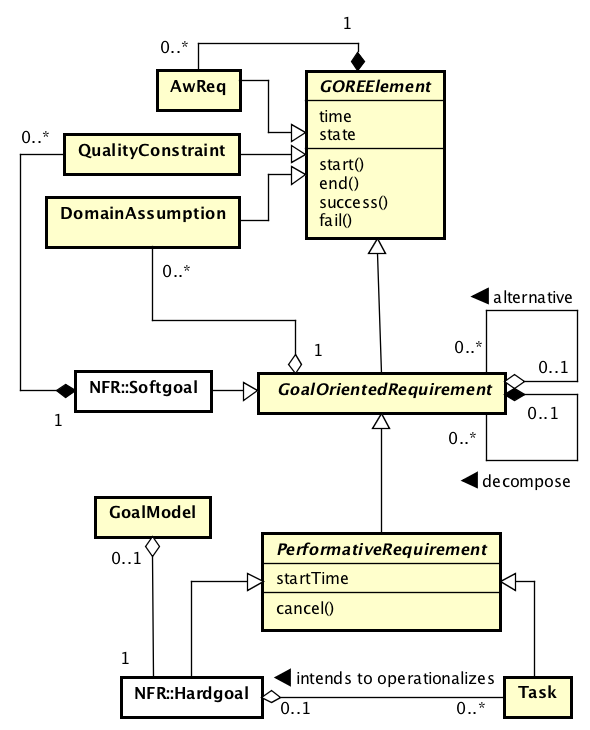
\includegraphics[width=0.7\textwidth]{figuras/metamodelos/metamodelo-zanshin-novo.png}
	\caption{Proposta de evolução do metamodelo do \framework \zanshin.}
	\label{figura-metamodelo-novo}
\end{figure}

\begin{itemize}
	\item A partir de agora, todos os elementos são especializações de \textit{GOREElement}, que passa a englobar características das antigas classes \textit{Requirement} e \textit{DefinableRequirement}, resolvendo então o problema~\ref{p2}. 

	\item A agregação pai/filho agora ocorre em dois tipos e acontece em um elemento mais específico: um requisito pode ser decomposto (\textit{decompose}) em outros, referindo-se assim a refinamentos do tipo ``E'', ou refinado através da agregação denominada ``alternative'', que trata de alternativas a um requisito, ou seja, refinamentos do tipo ``OU''. Dessa forma o metamodelo pode retratar melhor os tipos de refinamentos admitidos e quais são, exatamente, os componentes que  os aceitam. Além do mais, a partir desta melhoria os refinamentos acontecem somente nos elementos que especializam \textit{GoalOrientedRequirement}, ou seja, somente \textit{Hardgoals}, \textit{Softgoal} e \textit{Tasks}. Essa modificação soluciona o problema~\ref{p1}.
	
	\item \textit{Softgoal} e \textit{QualityConstraint} passam a se relacionar por meio de relação de decomposição e, portanto, também fica mais evidente que todo \textit{Softgoal} deve ser operacionalizado por pelo menos um \textit{QualityConstraint}, dando fim, assim, ao problema~\ref{p3}.
	
	\item Nessa proposta, \awreqs tem uma relação direta de composição com o \textit{GOREElement} logo, define-se que qualquer tipo de requisito no modelo pode conter elementos de adaptação, assim resolve-se o problema~\ref{p4}.
	
	\item No novo metamodelo, foi criada uma relação direta entre \textit{Tasks} e \textit{Hardgoals} (denominados anteriormente por \textit{Goals}), assim fica explícito o relacionamento entre esses dois elementos, sinalizando que objetivos são refinados em tarefas, que podem ser refinadas apenas nelas mesmas. Soluciona-se então o problema~\ref{p5}.
	
	\item Propõe-se, por fim, uma relação de agregação entre \textit{DomainAssumption} e \textit{GoalOrientedRequirement}, assim fica claro que \textit{Domain Assumptions} são elementos que interagem apenas com \textit{Hardgoals}, \textit{Softgoals} e \textit{Tasks}, findando o problema~\ref{p6}.
	
\end{itemize}

Uma observação importante que deve ser feita refere-se ao fato de que um elemento só pode conter refinamentos exclusivamente do tipo ``E'' (``AND'') ou exclusivamente do tipo ``OU'' (``OR''). Essa decisão tem por objetivo facilitar a leitura e interpretação do diagrama, e não compromete a representatividade do modelo pois assume-se que caso necessário, o modelador pode agrupar refinamentos do mesmo tipo em um objetivo, como exemplificado na Figura~\ref{figura-refinamentos}.

\begin{figure}
	\centering
	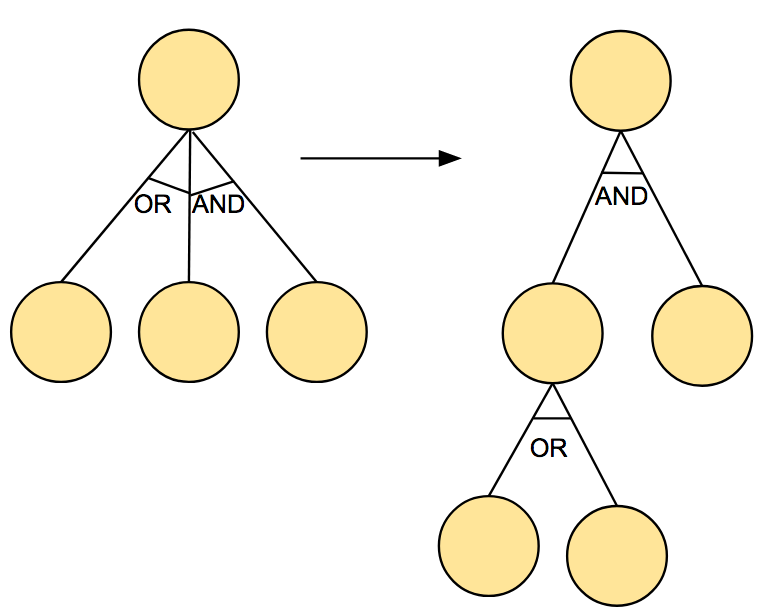
\includegraphics[width=0.7\textwidth]{figuras/metamodelos/exemplo-or-and.png}
	\caption{Exemplificação da representação de refinamentos no novo metamodelo.}
	\label{figura-refinamentos}
\end{figure}

%\vitor{A Figura~\ref{figura-refinamentos} ficaria ainda melhor se as bolinhas tivessem identificadores (genéricos, tipo E1, E2... E = Element), o que deixaria claro qual dos elementos na figura da direita é novo.}

%\vitor{Onde pode ser encontrado o código-fonte do novo Zanshin? Antes de você citar a URL do GitHub aqui, acho que deveríamos transferir o repositório para o NEMO. Pode ser?}